\section{Segway parameters}
\label{app:segwayParameters}
The purpose of this test is to measure the physical parameters describing the segway, namely the dimensions and masses of various parts of the segway.

\subsubsection{Equipment}
In \autoref{paramEqui}, the equipment used for performing the measurements is listed.

\begin{table}[H]
\centering
\scalebox{0.7}{
\begin{tabular}{|l|l|l|}
\hline
\bf{Name and type}           & \bf{AAU No.}  & \bf{ Remarks}   \\\hline
KERN - FCB 12K1 - Electronic & 86759         & 1 g precision \citep[p. 5]{weight}  \\\hline
Ruler                        & N/A           & 1 mm division   \\\hline
Caliper                      & N/A           & 0.1 mm division \\\hline
\end{tabular}
}
\caption{Equipment used for the test.}
\label{paramEqui}
\end{table}

\subsubsection{Procedure}
A blueprint of the segway with the measurement points can be seen in \autoref{segwaySchematic}.
The length measurements are performed using the ruler and calliper, where the values are read manually.
\begin{figure}[H]
\centering
	\begin{subfigure}[b]{0.35\textwidth}

	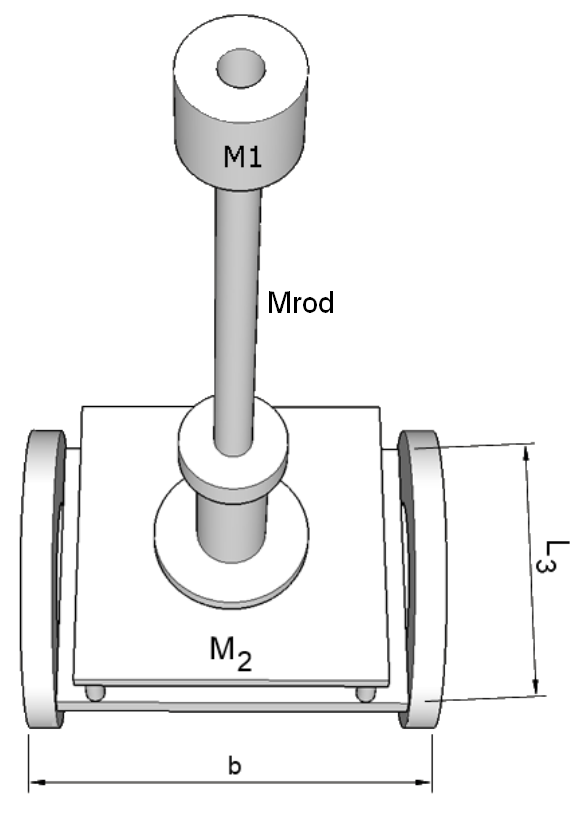
\includegraphics[width=\textwidth]{figures/segwayModelFront.png}
	\caption{The segway blueprint seen from the front.}
	\label{fig:segwayFront}
	\end{subfigure}
	\hspace{0.2\textwidth}
	~
	\begin{subfigure}[b]{0.25\textwidth}
	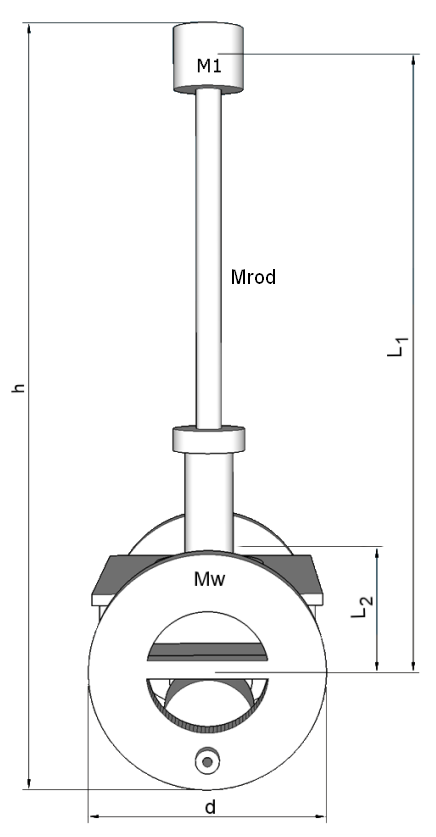
\includegraphics[width=\textwidth]{figures/segwayModelSide.png}
	\caption{The segway blueprint seen from the side.}
	\label{fig:segwaySide}
	\end{subfigure}
	\caption{A blueprint of the segway with parameter definitions \citep[p.~74]{DARSAS}.}
	\label{segwaySchematic}
\end{figure}


\subsubsection{Results}
The measurements of the relevant parameters is listed in \autoref{tab:dimensions}.

\begin{table}[H]
\centering
\scalebox{0.96}{
\rowcolors{1}{}{gray!10}
\begin{tabular}{|c|p{11cm}|c|c|}
\hline
\textbf{Symbol} & \textbf{Parameter} & \textbf{Value} & \textbf{Unit}\\\hline

$d$ & Wheel diameter & 117 & mm\\\hline
$h$ & Total height & 371 & mm \\\hline
$b$ & Total platform length & 174 & mm\\\hline
$L_1$ & Length from center of rotation to the center of the mass $M_p$ & 318 & mm \\\hline
$L_2$ & Distance from the pivot point to the center of mass & 57 & mm \\\hline
$L_3$ & Platform width & 90 & mm \\\hline
$m_p$ & Mass of cylindrical block at the top of the segway & 278 & g\\\hline
$m_c$ & Mass of the platform & 1323 & g \\\hline
$m_{rod}$ & Mass of the rod & 42 & g \\\hline
$m_w$ & Mass of each wheel & 133 & g \\\hline

\end{tabular}
}
\caption{Physical dimensions and massses of the segway parts.}\label{tab:dimensions}
\end{table}

\subsubsection{Conclusion}
The dimensions and masses of relevant parts of the segway have been measured. Any errors will most likely be due to reading errors of the measurements.